\documentclass[11pt]{article}

\usepackage{float}
\usepackage{hyperref}
\usepackage{graphicx}
% formatting
\usepackage{fullpage}
\usepackage{verbatim}
\usepackage{moreverb}
\usepackage{minted}
\usepackage{parskip}
\let\verbatiminput=\verbatimtabinput
\def\verbatimtabsize{4\relax}

\begin{document}
\title{EE142 Lab 0.5 - VNA Calibration}

\author{Vighnesh Iyer \\
Department of Electrical Engineering and Computer Sciences\\
College of Engineering, University of California, Berkeley}
\date{}
\maketitle

\section{Testing Cable Phase Stability}

\subsection{Two-Port Technique}
We connect a SMA cable between port 1 and 2. 

Before connecting the cable, the SMA connector's pin depth and dielectric depth are both checked and are within spec. Also, the SMA connector was examined under a stereo microscope and it was cleaned with a cotton swab and alcohol to remove surface contaminants (specks of dirt and metal fragments).

\begin{figure}[H]
	\minipage{0.50\textwidth}
	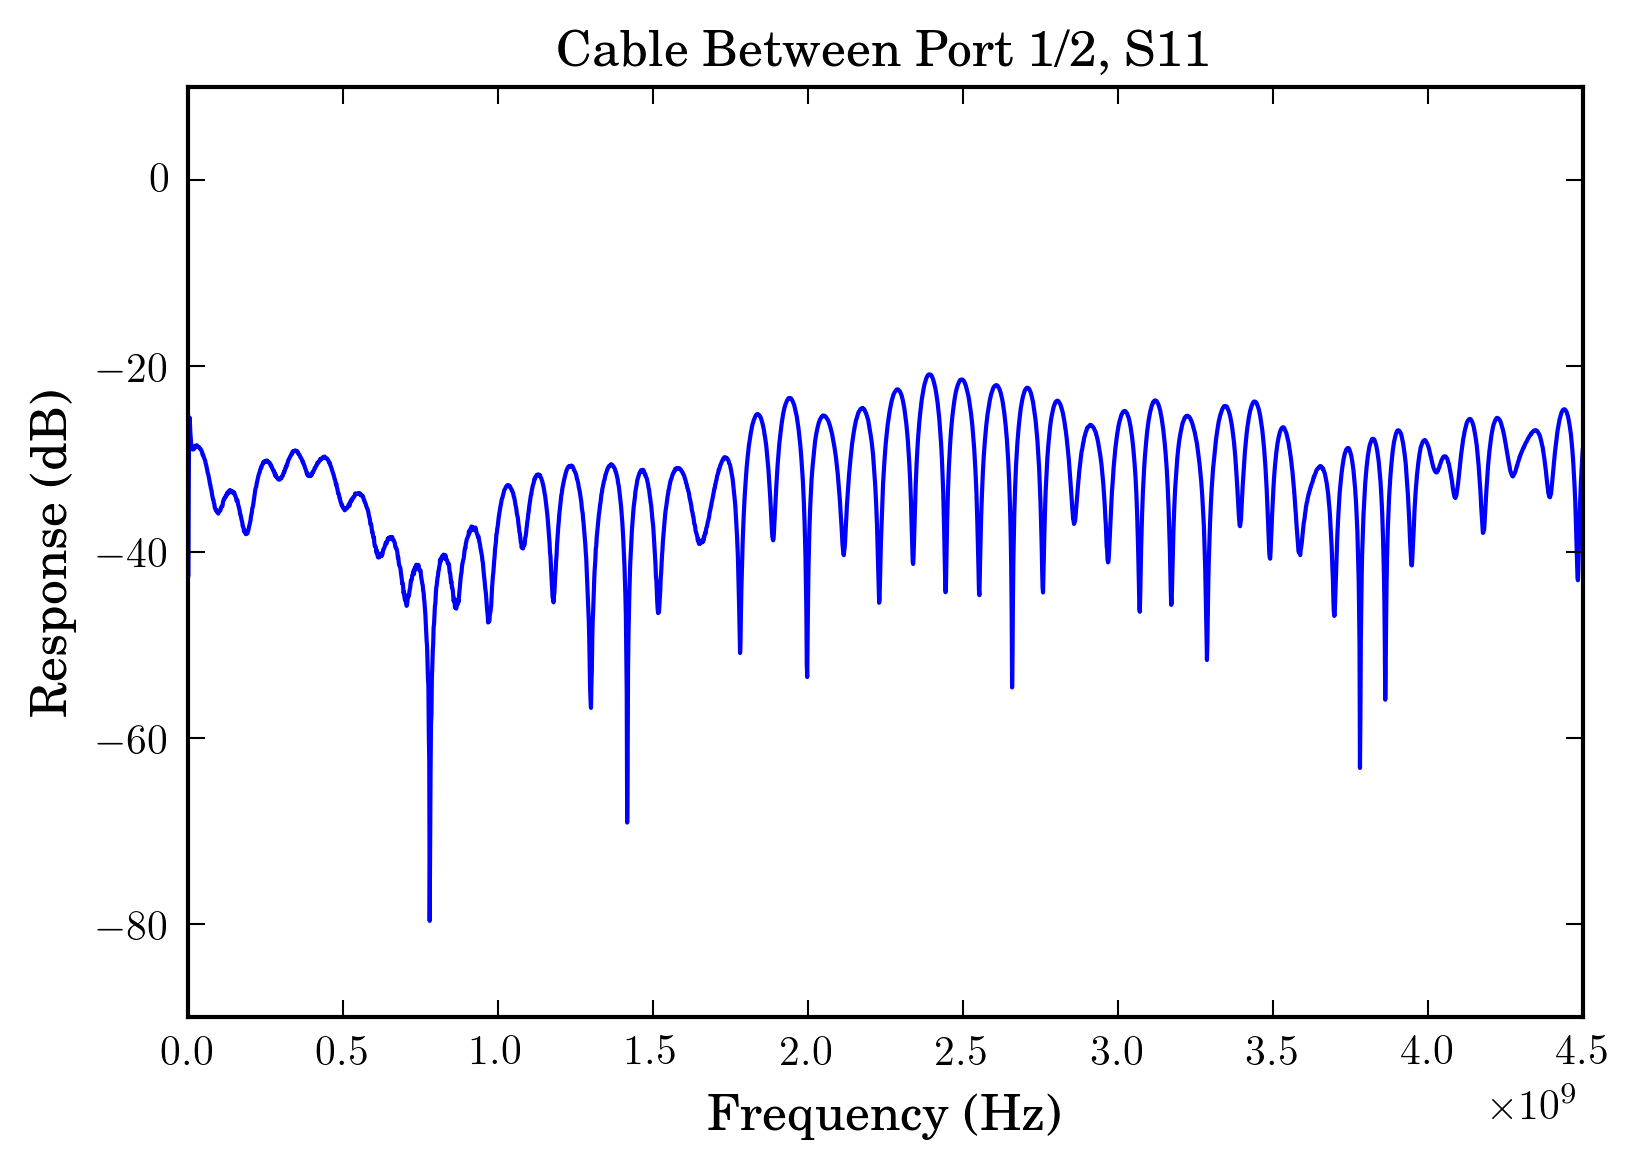
\includegraphics[width=\linewidth]{images/cable_phase_s11.png}
	\endminipage\hfill
	\minipage{0.50\textwidth}
	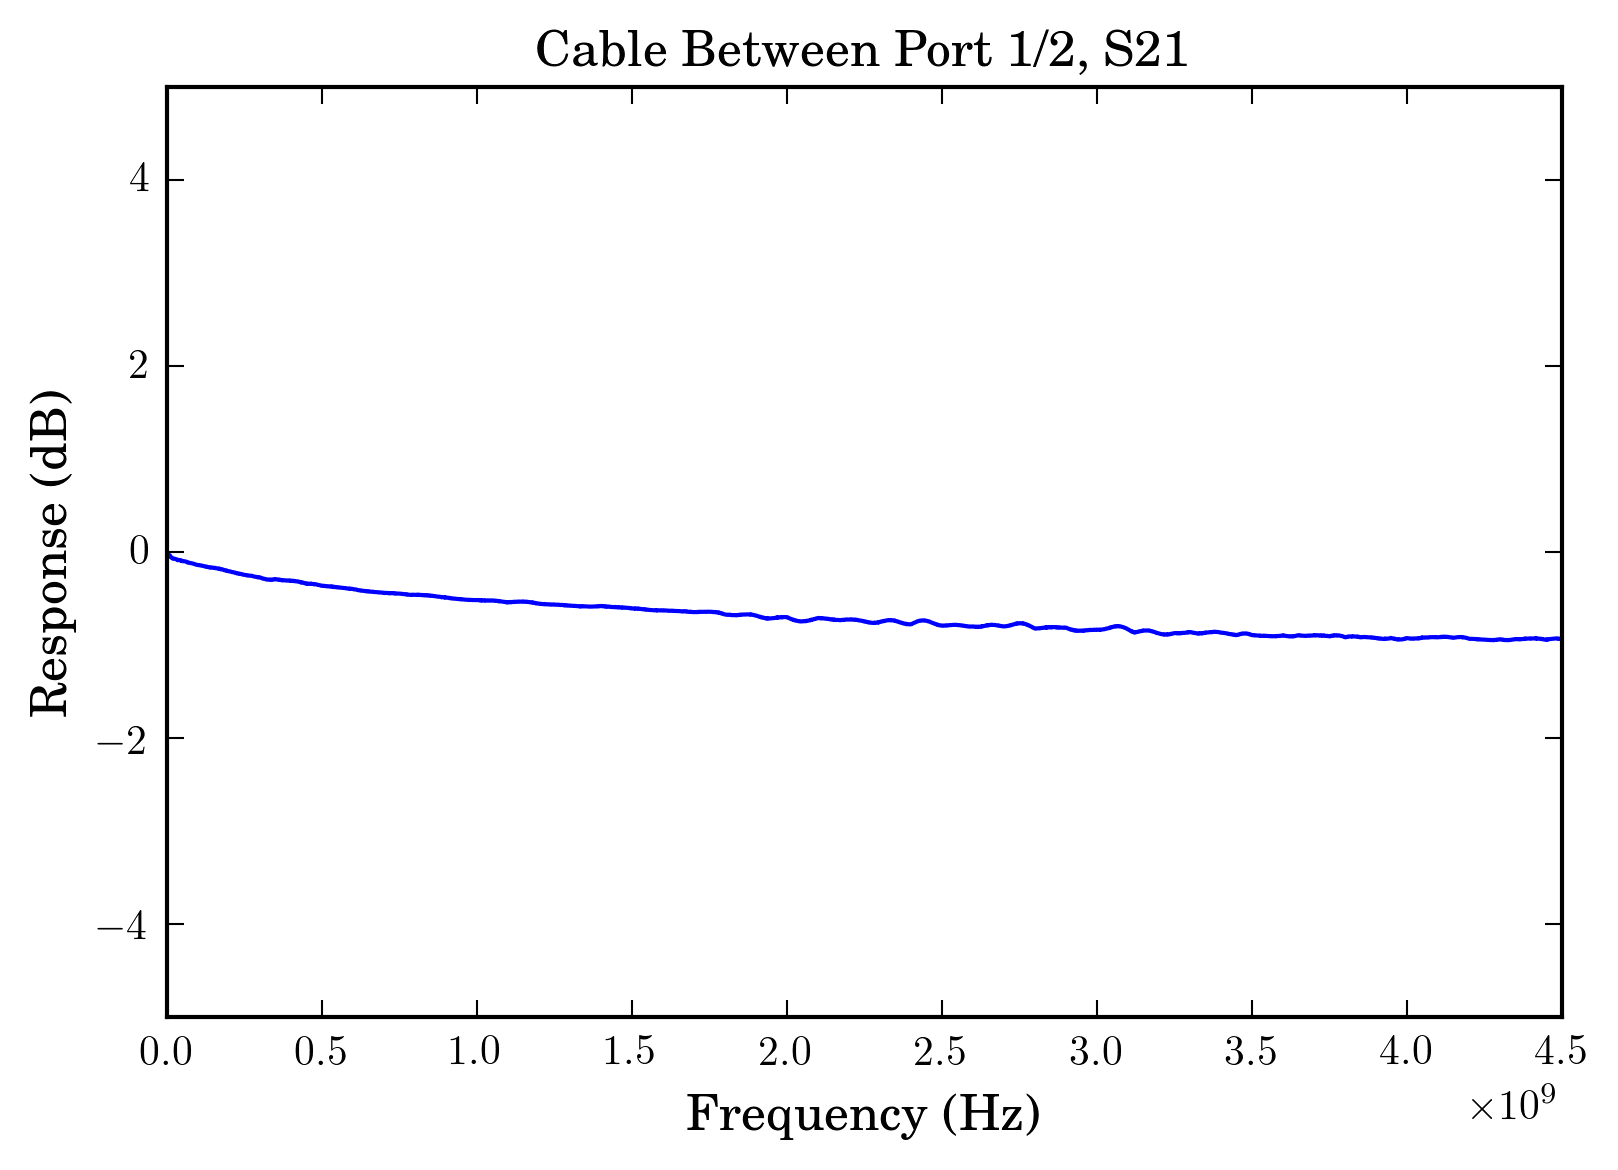
\includegraphics[width=\linewidth]{images/cable_phase_s21.png}
	\endminipage
\end{figure}

When plotting $S_{11}$, we see reflections and re-reflections 20 dB down which show discontinuities in the cable's impedance. When measuring $S_{21}$, we see that almost all the delivered power from port 1 makes its way to port 2 and we only see some drop-off at higher frequencies.


We then look at the phase of $S_{21}$. As expected, the phase wraps around several times for its given length. We then divide the current trace by the last captured trace using the \verb|Data/Memory| function of the NA. Both plots are shown.

\begin{figure}[H]
	\minipage{0.50\textwidth}
	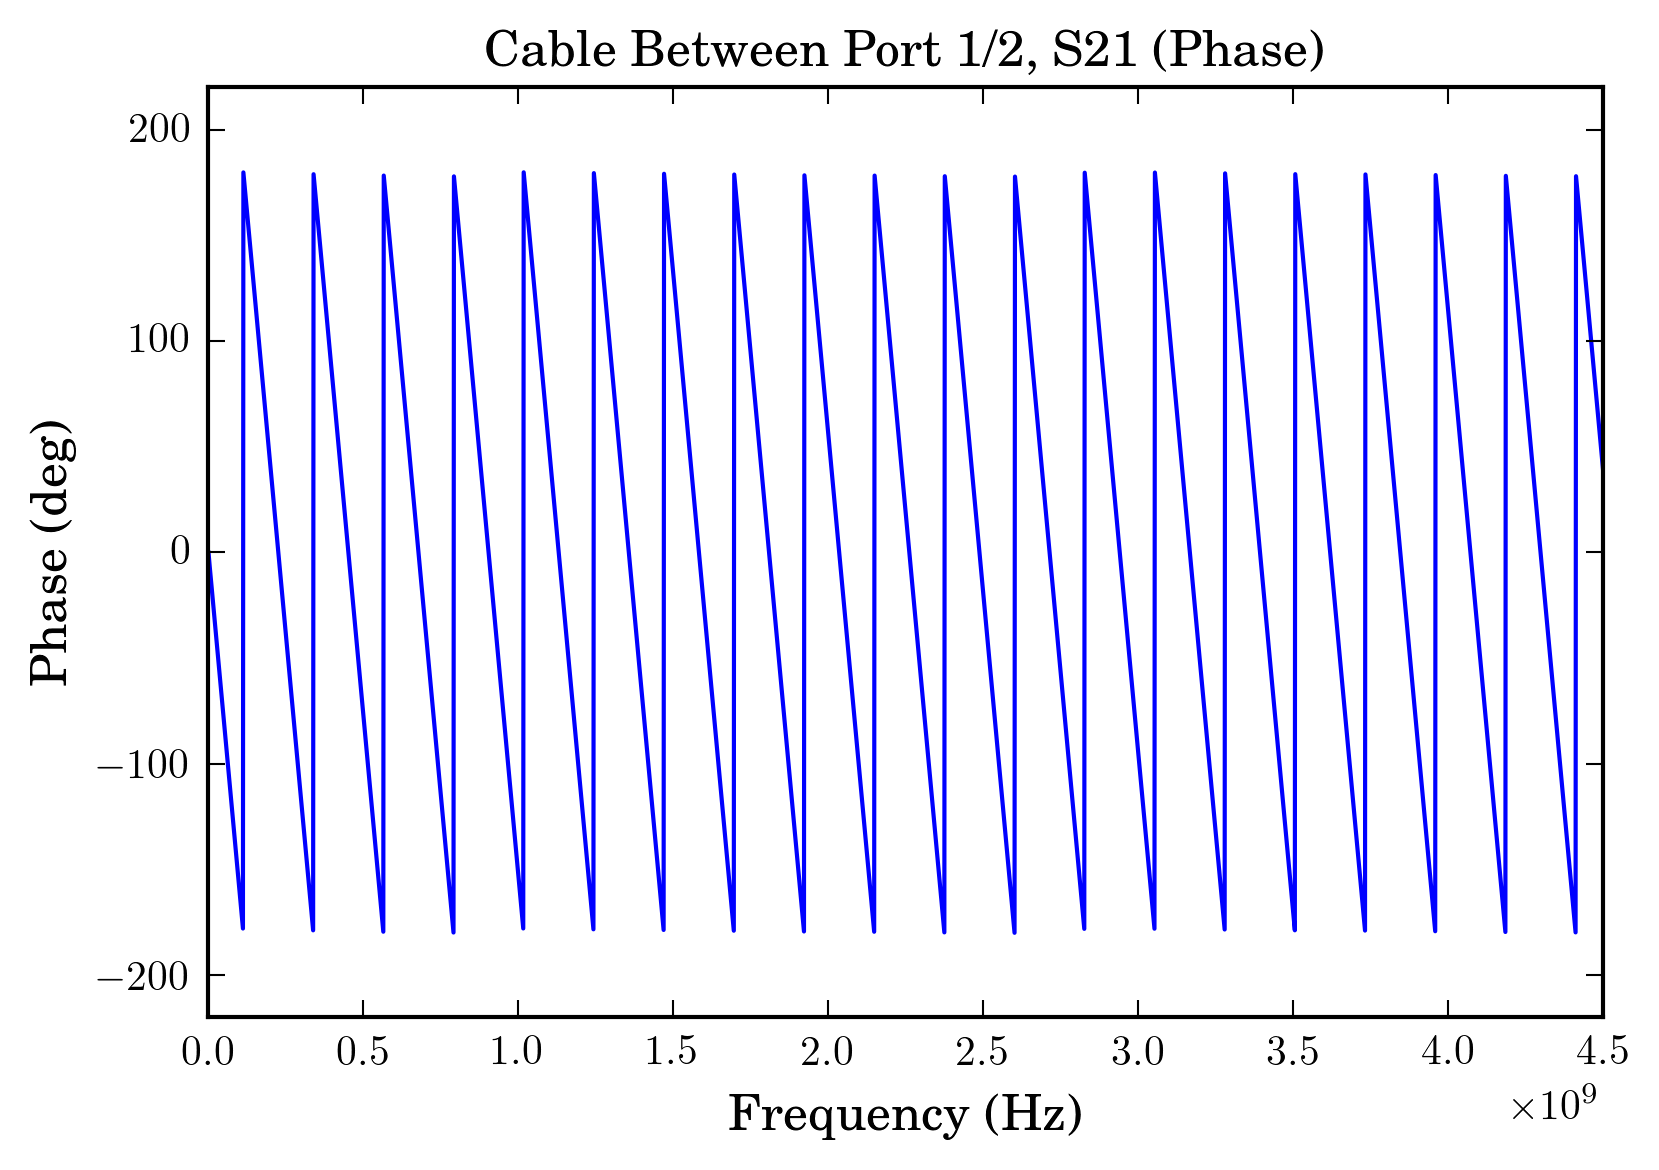
\includegraphics[width=\linewidth]{images/cable_phase_s21_phase.png}
	\endminipage\hfill
	\minipage{0.50\textwidth}
	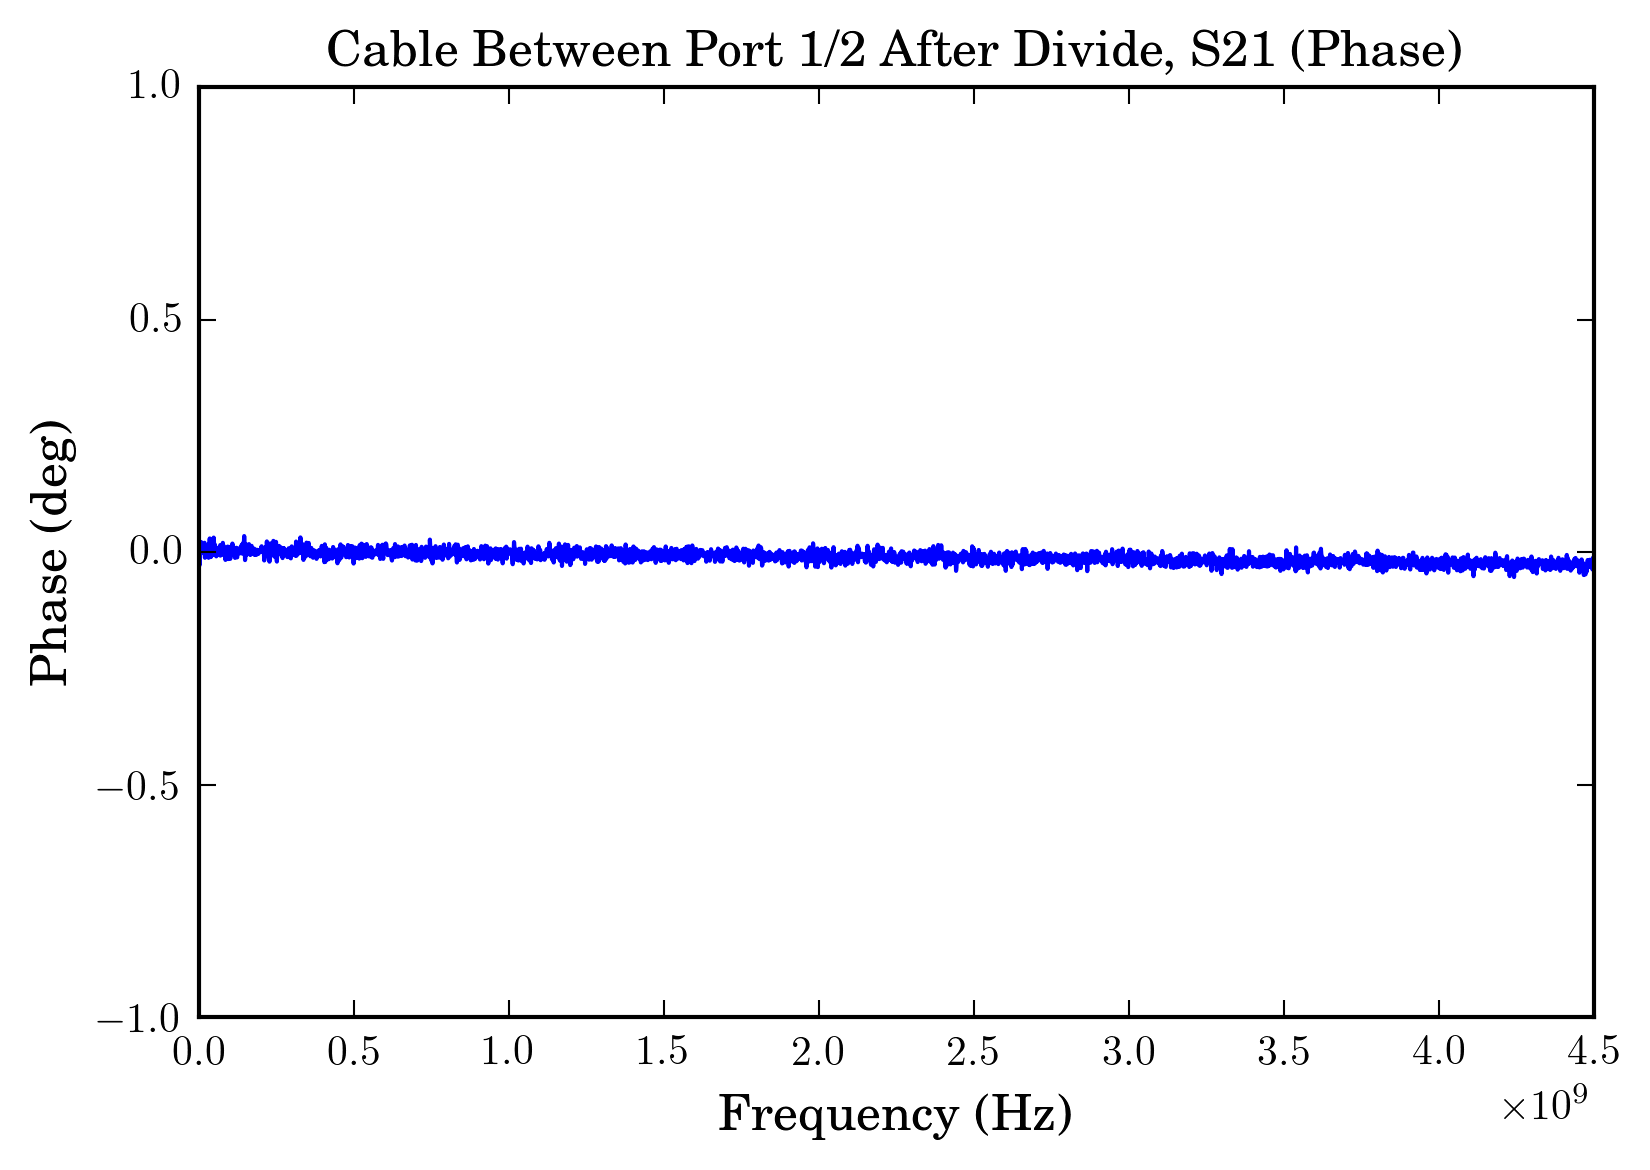
\includegraphics[width=\linewidth]{images/cable_phase_s21_after_data_divide.png}
	\endminipage
\end{figure}

Now, we wiggle and bend the cable several times. The phase of the cable changes due to changes in its electrical length. After some movement, we let the cable sit on the lab bench again until the phase trace settles.

\begin{figure}[H]
	\centering 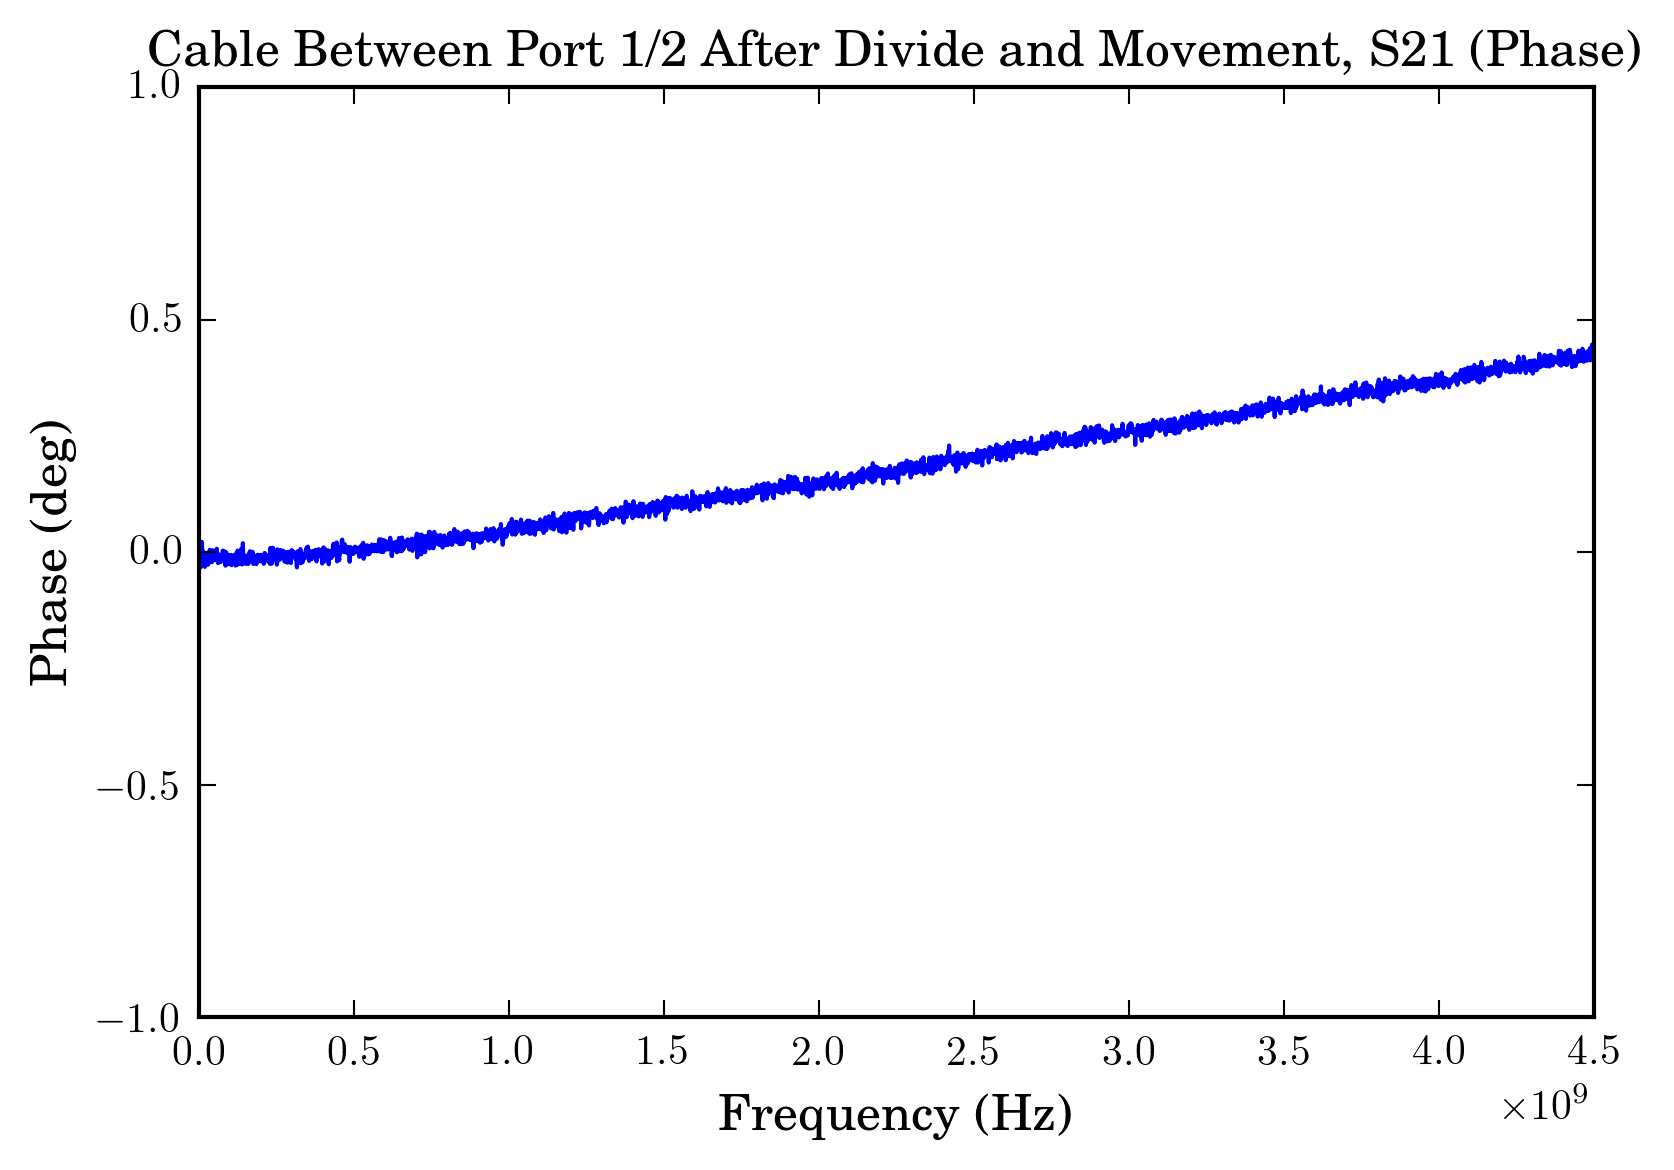
\includegraphics[width=\linewidth-7cm]{images/cable_phase_s21_after_movement.png}
\end{figure}

We see some positive phase on the upper frequencies, but only less than 0.5 degrees. This cable seems to have decent phase stability.

\subsection{One-Port with Cal Standard Technique}

We connect one end of a SMA cable to port 1 and the other end to a open calibration standard. The display is set to Log-Mag $S_{11}$.

The cable is placed down and we use the \verb|Data->Mem| = \verb|Data-Mem| to subtract out the last captured trace from the current trace. This pushes the Log-Mag trace to around -60 dB, but I expected the trace to plunge further down to -80 dB closer to the noise floor of the instrument.

\begin{figure}[H]
	\centering 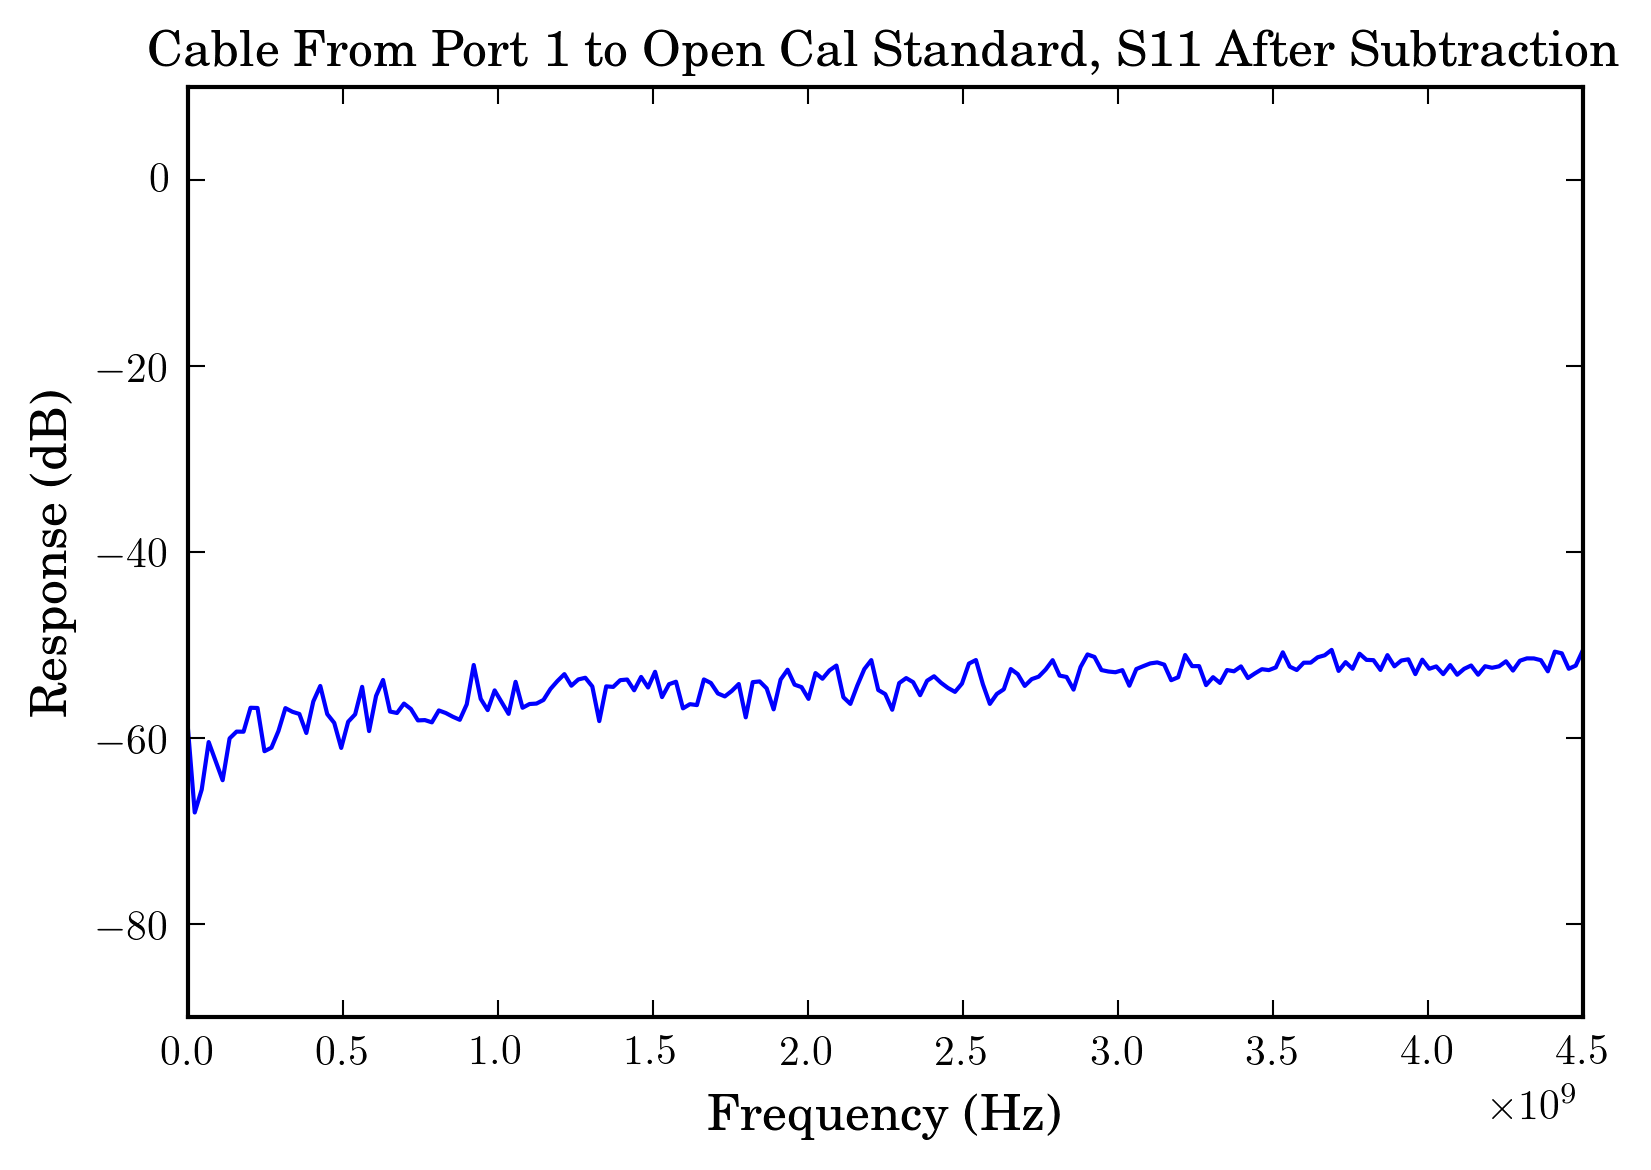
\includegraphics[width=\linewidth-6cm]{images/one_port_s11_open_cal.png}
\end{figure}

Finally, the cable is moved around and flexed for 10 seconds, and the cable is placed down on the lab bench again. The trace is allowed to settle down.

\begin{figure}[H]
	\centering 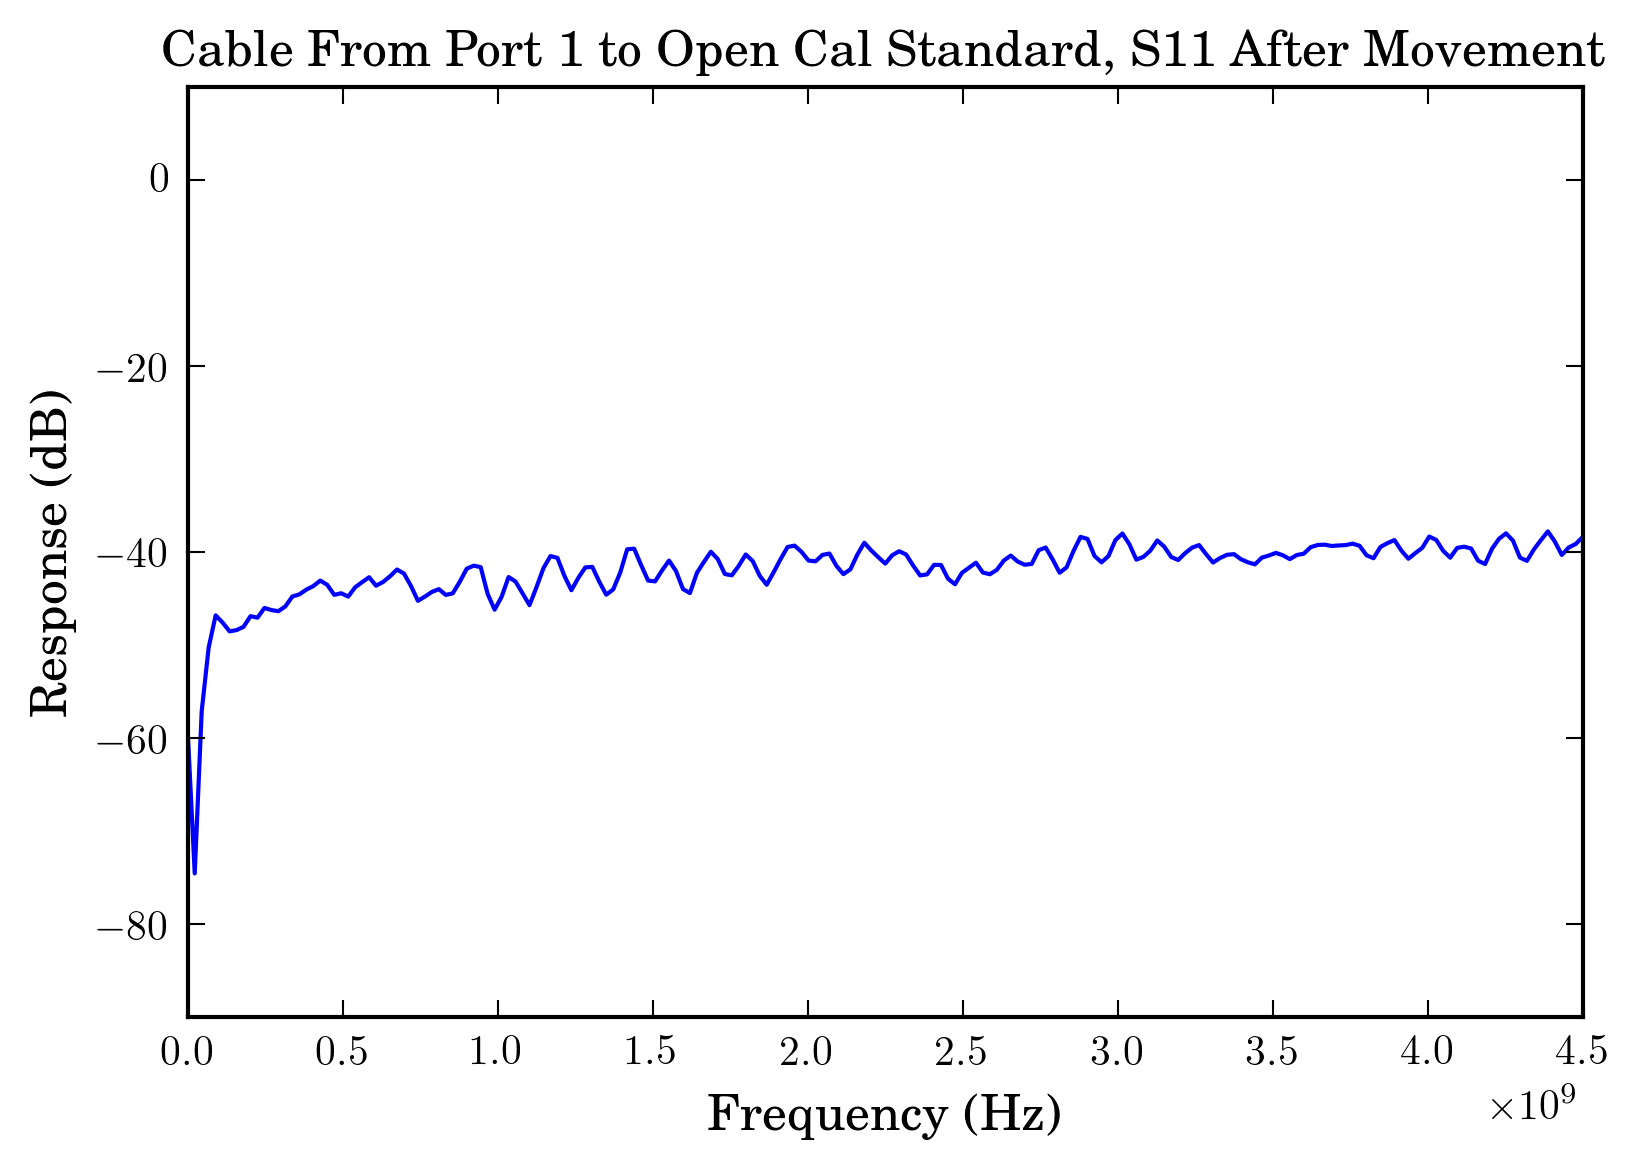
\includegraphics[width=\linewidth-6cm]{images/one_port_s11_open_cal_after_movement.png}
\end{figure}

The trace should have moved from its -80 dB state upwards as the cable's electrical length/phase has been slightly changed due to the movement. A very good cable moves to around -50 dB, while a decent cable moves to around -40 dB. A poor cable will move up to -30 dB or higher.

We can see that our chosen cable is of mid-range quality and has enough phase stability to perform reliable measurements.

\section{Calibration using E-Cal}

I performed a one-port calibration using the SOL standards first, but I found that they gave inconsistent results and didn't give a good cal when testing other standards.

I decided to then try the E-Cal, which was easy to set up to calibrate the VNA, with the same set of cables I tested earlier. I performed a full two-port cal.

Here is a Smith chart and $S_{11}$ trace of a open standard directly connected to port 1 (no cable) before E-Cal calibration.

\begin{figure}[H]
	\centering 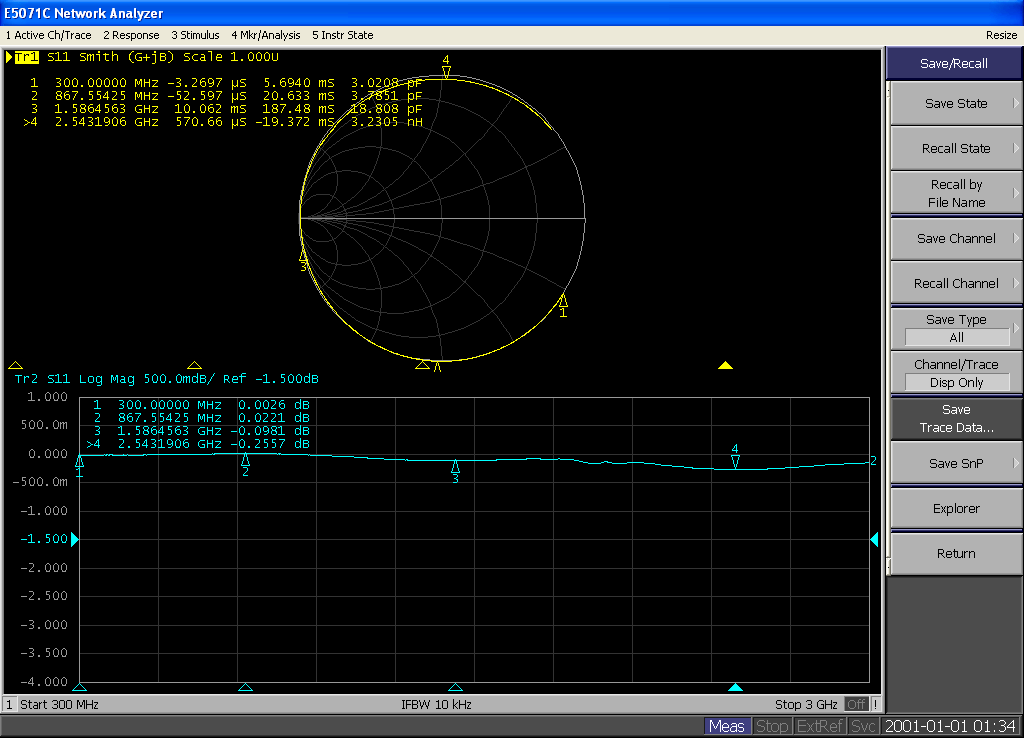
\includegraphics[width=\linewidth-6cm]{images/S11_OPEN_STD_BEFORE_CAL.PNG}
\end{figure}

We can see that the electrical delay isn't compensated for and the open doesn't look perfect.

\section{Verifying Calibration With Cal Standards}
After E-Cal calibration with the set of cables I used earlier, I tried connecting an open standard to the end of the cable to check the calibration quality.

\begin{figure}[H]
	\centering 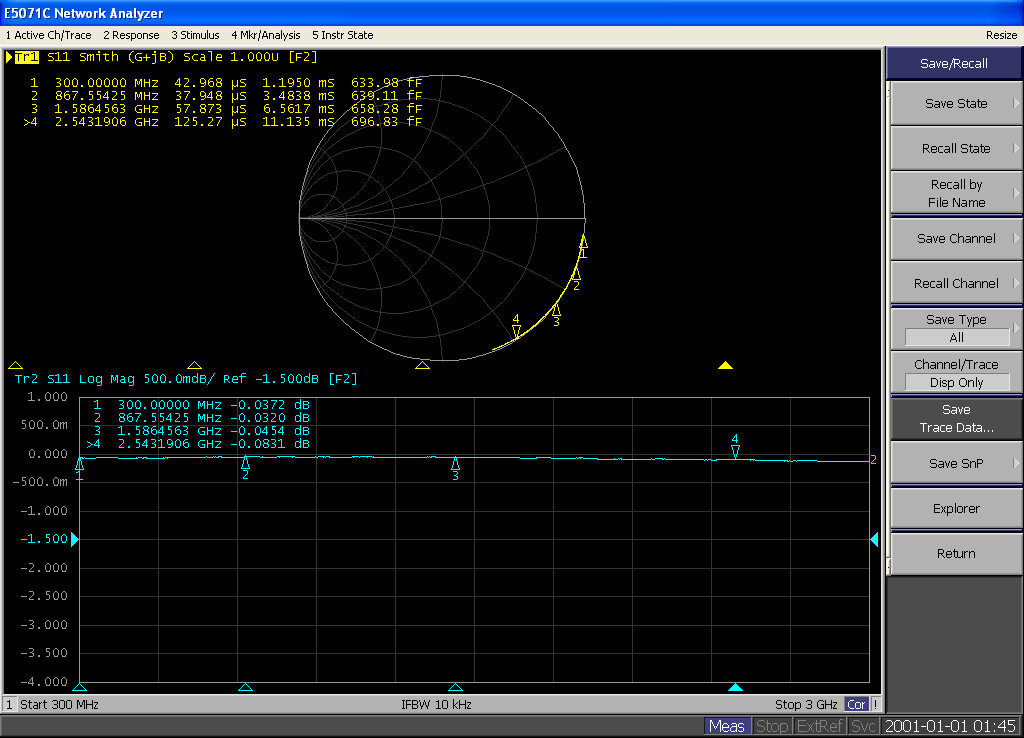
\includegraphics[width=\linewidth-6cm]{images/S11_OPEN_STD_AFTER_CAL.PNG}
\end{figure}

This looks a lot better, and the only issue is the electrical delay of the open standard isn't factored into the measurement. Otherwise, it looks nearly perfect.

Comparing it to the reference from the Calibration powerpoint:

\begin{figure}[H]
	\centering 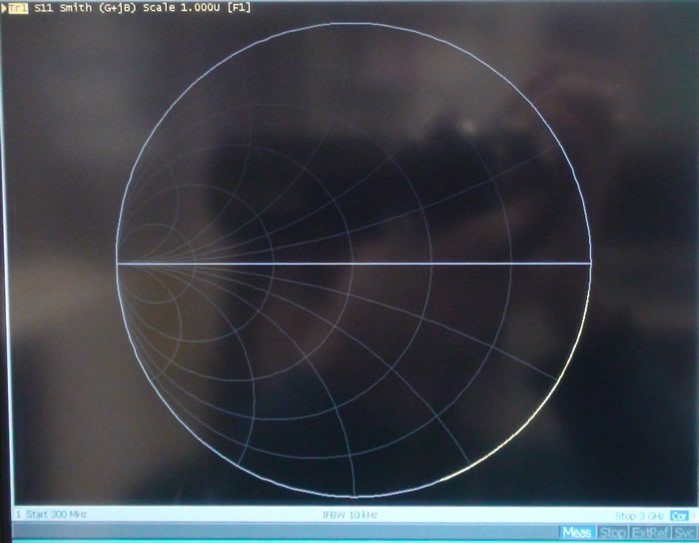
\includegraphics[width=\linewidth-6cm]{images/S11_OPEN_STD_REFERENCE.JPG}
\end{figure}

We can see that it is a very close match before accounting for offset delay and the cable I used not being held perfectly still.

\end{document}
